%% LyX 2.2.4 created this file.  For more info, see http://www.lyx.org/.
%% Do not edit unless you really know what you are doing.
\documentclass[english]{article}
\usepackage{lmodern}
\usepackage[T1]{fontenc}
\usepackage[latin9]{inputenc}
\usepackage{geometry}
\geometry{verbose,tmargin=2cm,bmargin=2.5cm,lmargin=2.5cm,rmargin=2.5cm}
\usepackage{textcomp}
\usepackage{amstext}
\usepackage{amsmath}
\usepackage{amssymb}
\usepackage{graphicx}
\usepackage{comment}
\usepackage{titlesec}
\titlespacing*{\section}{0pt}{2.4ex plus 0.7ex minus 0.2ex}{1.6ex plus 0.2ex}
\titlespacing*{\subsection}{0pt}{2.3ex plus 0.7ex minus 0.2ex}{1.0ex plus 0.1ex}
\titlespacing*{\subsubsection}{0pt}{1.8ex plus 0.5ex minus 0.2ex}{0.7ex plus 0.1ex}

\makeatletter

\begin{comment}
First make sure uve read the relevant files: this latex doc, coursework.pdf, coursework.ipynb, code.py

This latex document details all the lab report for 3F8 inference
Try to always include core mathematics where relevant, make sure notations are consistent throughout
Instructions are in coursework.pdf, make sure to answer the questions comprehensively in this latex doc
The relevant ipynb file is coursework.ipynb and code.py in the /3F8 folder, but try to make sure outputs are cleared before further processing to save tokens
Make sure all vectors are bolded
Make sure all math is explained comprehensively and clearly
ALWAYS try to make minimal edits to existing ipynb notebooks, especially if they contain reusable functions - try to reuse them as much as possible making small modifications
LLM tips: you can refer to the logistic regression notes "C:\FUTURE\Eng2A\3F8\handout4-classification-slides.pdf" if needed

\end{comment}


%%%%%%%%%%%%%%%%%%%%%%%%%%%%%% LyX specific LaTeX commands.
%% Because html converters don't know tabularnewline
\providecommand{\tabularnewline}{\\}

\makeatother

\usepackage{babel}
\begin{document}

\title{3F8: Inference: Short Lab Report}

\author{Zihe Liu | zl559}
\maketitle
\begin{abstract}
    We implement a logistic classifier and apply it to a binary
    classification dataset with non-linearly separable classes.
    We derive the gradient of the log-likelihood, train the model
    using gradient ascent, and evaluate performance via log-likelihoods
    and confusion matrices. We then improve the classifier by expanding
    the inputs through Gaussian radial basis functions (RBFs) and
    investigate how the RBF width $l$ governs the bias--variance
    trade-off. The best-performing model ($l = 0.1$) achieves a test
    log-likelihood of $-0.35$, a substantial improvement over the
    linear baseline ($-0.66$).
\end{abstract}

\section*{Introduction}

Classification is a fundamental task in machine learning: given
labelled training data, the goal is to learn a mapping from inputs to
discrete class labels that generalises to unseen data. Logistic
regression is a simple yet principled approach that models class
probabilities via the sigmoid function applied to a linear combination
of input features, yielding a linear decision boundary. However, many
real-world datasets are not linearly separable.

In this report, we first derive and implement the logistic classifier,
then demonstrate its limitations on a non-linearly separable dataset.
We subsequently introduce a non-linear feature expansion using Gaussian
radial basis functions (RBFs) and investigate how the RBF width
parameter $l$ affects model learning and performance.

\section*{Exercise a): Gradients of Log-Likelihood\label{sec:Exercise-a}}

We derive the gradient of the log-likelihood
with respect to the parameter vector $\boldsymbol{\beta}$,
given a vector of binary labels $\mathbf{y}$ and a matrix of input
features $\mathbf{X}$. The probability of
a positive class label is given by the logistic (sigmoid) function
$\sigma(a) = 1/(1+e^{-a})$ applied to the activations:
\[
    P(y^{(n)} = 1 \mid \tilde{\mathbf{x}}^{(n)})
    = \sigma(\boldsymbol{\beta}^{T}\tilde{\mathbf{x}}^{(n)})\,,
    \qquad
    P(y^{(n)} = 0 \mid \tilde{\mathbf{x}}^{(n)})
    = 1 - \sigma(\boldsymbol{\beta}^{T}\tilde{\mathbf{x}}^{(n)})
\]
where $\tilde{\mathbf{x}}^{(n)} = (1, \mathbf{x}^{(n)})^{T}$ are the bias-augmented
inputs, so that $\boldsymbol{\beta}^{T}\tilde{\mathbf{x}}^{(n)}
    = \beta_0 + \sum_{d=1}^{D}\beta_d x_d^{(n)}$.
These two cases can be written compactly as a single Bernoulli likelihood:
\[
    P(y^{(n)} \mid \tilde{\mathbf{x}}^{(n)}, \boldsymbol{\beta})
    = \sigma(\boldsymbol{\beta}^{T}\tilde{\mathbf{x}}^{(n)})^{y^{(n)}}
    \left(1 - \sigma(\boldsymbol{\beta}^{T}\tilde{\mathbf{x}}^{(n)})\right)^{1 - y^{(n)}}
\]
Assuming the $N$ datapoints are independent and identically distributed,
the dataset log-likelihood is:
\[
    \mathcal{L}(\boldsymbol{\beta})
    = \log P(\mathbf{y} \mid \mathbf{X}, \boldsymbol{\beta})
    = \sum_{n=1}^{N}\left[
    y^{(n)}\log\sigma(\boldsymbol{\beta}^{T}\tilde{\mathbf{x}}^{(n)})
    + (1-y^{(n)})\log\left(1-\sigma(\boldsymbol{\beta}^{T}\tilde{\mathbf{x}}^{(n)})\right)
    \right]
\]
Let $a^{(n)} = \boldsymbol{\beta}^{T}\tilde{\mathbf{x}}^{(n)}$, so that
$\frac{\partial a^{(n)}}{\partial \boldsymbol{\beta}} = \tilde{\mathbf{x}}^{(n)}$. Noting the derivative of the logistic function $\frac{d\sigma(a)}{da} = \sigma(a)\left(1 - \sigma(a)\right)$,
\[
    \frac{\partial}{\partial\boldsymbol{\beta}}\left[y^{(n)}\log\sigma(a^{(n)})\right]
    = y^{(n)} \cdot \frac{1}{\sigma(a^{(n)})}
    \cdot \underbrace{\frac{d\sigma}{da}}_{\sigma(1-\sigma)}
    \cdot \underbrace{\frac{\partial a^{(n)}}{\partial \boldsymbol{\beta}}}_{\tilde{\mathbf{x}}^{(n)}}
    = y^{(n)}\left(1 - \sigma(a^{(n)})\right)\tilde{\mathbf{x}}^{(n)}
\]
\[
    \frac{\partial}{\partial\boldsymbol{\beta}}\left[(1-y^{(n)})\log(1 - \sigma(a^{(n)}))\right]
    = (1 - y^{(n)}) \cdot \frac{-\sigma(a^{(n)})(1-\sigma(a^{(n)}))}{1 - \sigma(a^{(n)})}
    \cdot \tilde{\mathbf{x}}^{(n)}
    = -(1-y^{(n)})\sigma(a^{(n)})\tilde{\mathbf{x}}^{(n)}
\]
Combining these two contributions for datapoint $n$:
\begin{align*}
     & y^{(n)}(1 - \sigma(a^{(n)}))\tilde{\mathbf{x}}^{(n)}
    - (1 - y^{(n)})\sigma(a^{(n)})\tilde{\mathbf{x}}^{(n)}
    = \left(y^{(n)} - \sigma(a^{(n)})\right)\tilde{\mathbf{x}}^{(n)}
\end{align*}
Summing over all $N$ datapoints,
\[
    \boxed{\frac{\partial\mathcal{L}(\boldsymbol{\beta})}{\partial\boldsymbol{\beta}}
        = \sum_{n=1}^{N}\left(y^{(n)}
        - \sigma(\boldsymbol{\beta}^{T}\tilde{\mathbf{x}}^{(n)})\right)\tilde{\mathbf{x}}^{(n)}
        = \tilde{\mathbf{X}}^{T}\left(\mathbf{y} - \boldsymbol{\sigma}\right)}
\]
where $\tilde{\mathbf{X}}$ is the $N \times (D+1)$ matrix whose $n$-th row
is $(\tilde{\mathbf{x}}^{(n)})^{T}$, and $\boldsymbol{\sigma}$ is the
$N$-dimensional vector with entries
$\sigma(\boldsymbol{\beta}^{T}\tilde{\mathbf{x}}^{(n)})$.
The vectorised form follows because the sum
$\sum_n (\cdot)\tilde{\mathbf{x}}^{(n)}$ is equivalent to the matrix product
$\tilde{\mathbf{X}}^T$ applied to the residual vector
$(\mathbf{y} - \boldsymbol{\sigma})$.


\section*{Exercise b) Vectorized Gradient Ascent}

In this exercise we write vectorised pseudocode to estimate the
parameters $\boldsymbol{\beta}$ using gradient ascent of the log-likelihood.
The update rule is
\[
    \boldsymbol{\beta}^{(\text{new})}
    = \boldsymbol{\beta}^{(\text{old})}
    + \eta \left.\frac{\partial\mathcal{L}(\boldsymbol{\beta})}{\partial\boldsymbol{\beta}}\right|_{\boldsymbol{\beta}=\boldsymbol{\beta}^{(\text{old})}}
    = \boldsymbol{\beta}^{(\text{old})}
    + \eta\, \tilde{\mathbf{X}}^{T}\left(\mathbf{y}
    - \boldsymbol{\sigma}^{(\text{old})}\right),
\]
where $\boldsymbol{\sigma}^{(\text{old})}$ is the vector of predictions
$\sigma(\boldsymbol{\beta}^{(\text{old})T}\tilde{\mathbf{x}}^{(n)})$
under the current parameters.
The pseudocode is as follows:
\begin{verbatim}
Function estimate_parameters:

   Input:  feature matrix X (N x D), labels y (N x 1),
           learning rate eta, number of iterations T
   Output: vector of coefficients b ((D+1) x 1)

   Code:
      X_tilde = [ones(N,1), X]        % augment with bias column
      b = randn(D+1, 1)               % initialise randomly

      for t = 1 to T:
          sigma = 1 / (1 + exp(-X_tilde * b))   % predictions (N x 1)
          grad = X_tilde^T * (y - sigma)         % gradient ((D+1) x 1)
          b = b + eta * grad                     % gradient ascent step

      return b
\end{verbatim}
The learning rate $\eta$ should be chosen small enough that the log-likelihood
increases roughly monotonically, but large
enough that convergence is achieved within a reasonable number of iterations.
The number of iterations $T$ should be large enough for the log-likelihood to
plateau.

\section*{Exercise c) Data Visualisation}

The dataset consists of $N = 1000$ datapoints with two-dimensional input
features $\mathbf{x}^{(n)} \in \mathbb{R}^2$ and binary class labels
$y^{(n)} \in \{0, 1\}$. From Figure~\ref{fig:data_visualisation}, we observe that Class 2 (blue) is concentrated in the upper and lower area of the input space, while Class 1 (red) is interspersed  between the 2 blue regions. The two classes overlap significantly, particularly around the boundaries, and no single straight line can cleanly separate them. A linear classifier produces a decision boundary of the form $\boldsymbol{\beta}^T \tilde{\mathbf{x}} = 0$, which is a straight line in 2D. Given the non-linear arrangement of the classes, such a linear boundary would inevitably misclassify a substantial portion of the data. A non-linear decision boundary would be needed to capture the true class structure more accurately.

\begin{figure}[h]
    \begin{centering}
        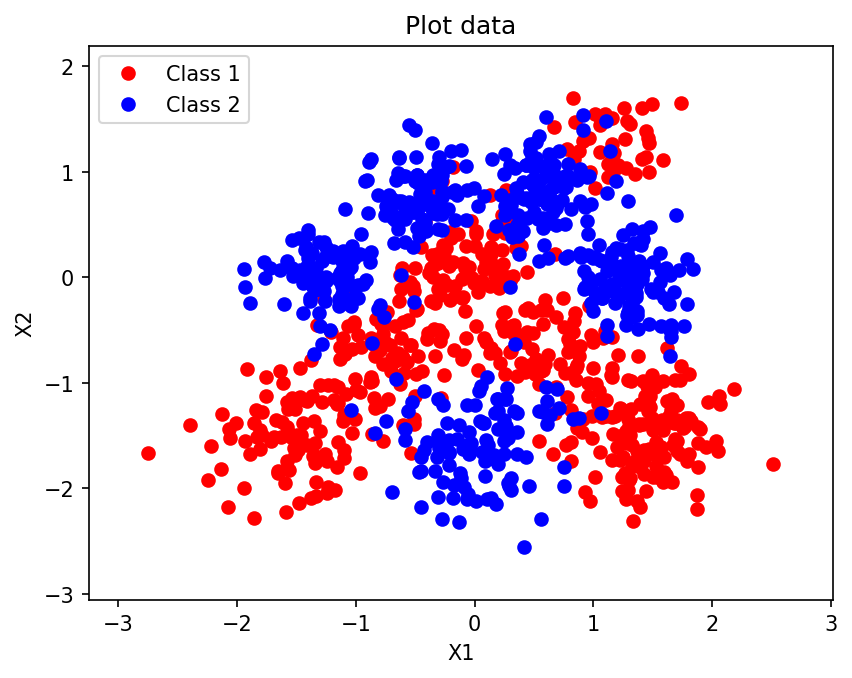
\includegraphics[width=0.25\paperwidth]{figures/data_visualisation.png}
        \par\end{centering}
    \caption{Visualisation of the dataset in the $(X_1, X_2)$ input space.
        Red points are Class 1 ($y=0$) and blue points are Class 2 ($y=1$).
        \label{fig:data_visualisation}}
\end{figure}




\section*{Exercise d) Training the Linear Classifier}

The data is split randomly\footnote{A fixed numpy random seed of 1 was used for reproducibility.} into training ($N_{\text{train}} = 800$)
and test ($N_{\text{test}} = 200$) sets. Gradient ascent is implemented as:
\begin{verbatim}
sigmoid_value = predict(X_tilde_train, w)
w = w + alpha * np.dot(X_tilde_train.T, y_train - sigmoid_value)
\end{verbatim}
We train the classifier with learning rate $\eta = 0.0005$ for $T = 100$
iterations. The average log-likelihood on the training and test sets as
the optimisation proceeds is shown in Figure~\ref{fig:learning_curves}.

\begin{figure}[h]
    \begin{centering}
        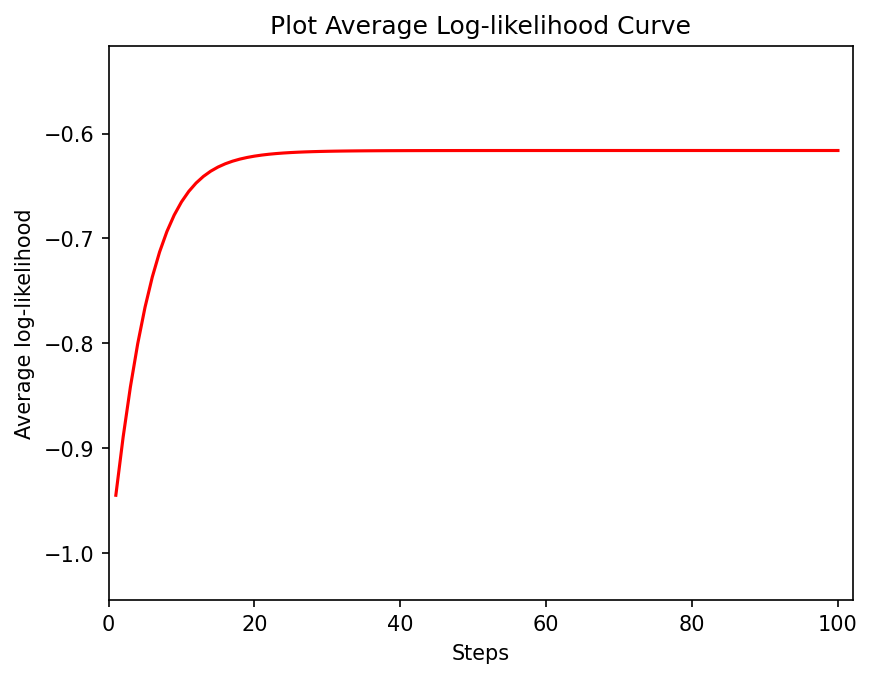
\includegraphics[width=0.2\paperwidth]{figures/ll_train_linear.png}\hspace{1cm}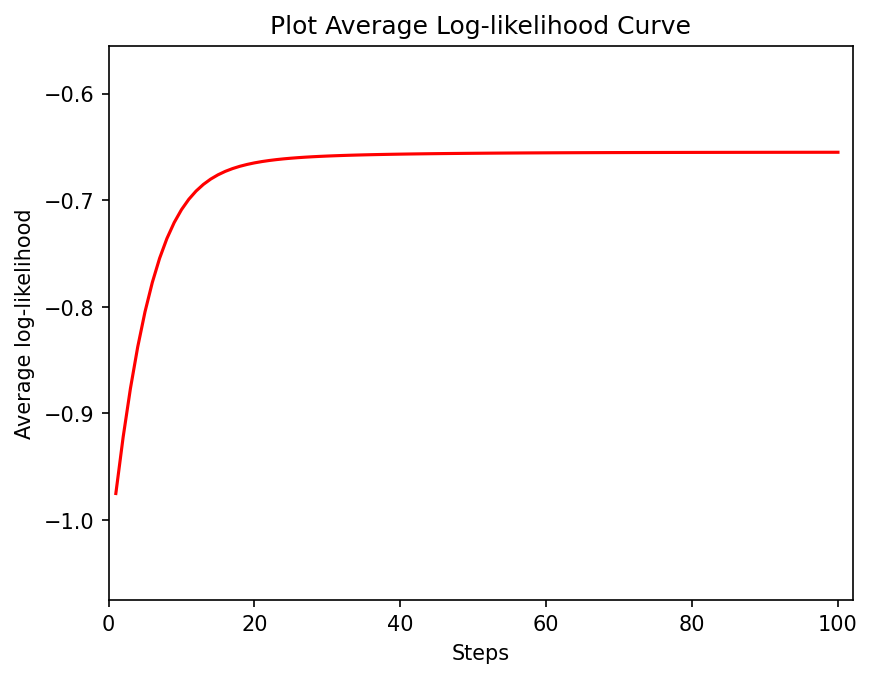
\includegraphics[width=0.2\paperwidth]{figures/ll_test_linear.png}
        \par\end{centering}
    \caption{Learning curves showing the average log-likelihood per datapoint
        on the training (left) and test (right) datasets.\label{fig:learning_curves}}
\end{figure}

Both curves increase monotonically and plateau after approximately 20
iterations, indicating that the optimisation has converged and
$\eta = 0.0005$ is an appropriate learning rate.
The training and test curves follow a similar trajectory, suggesting
there is no overfitting -- as expected for a model with only $D+1 = 3$
parameters fitting 800 datapoints.

Figure~\ref{fig:contours_linear} displays the contours of the
predictive probabilities overlaid on the data. The contours are parallel straight lines, confirming the linear nature of the decision boundary. The $0.5$ contour (the decision boundary) runs roughly diagonally, separating the upper region (higher
$P(y=1)$) from the lower region. However, as anticipated in Exercise c),
a linear boundary cannot capture the non-linear class structure: many
red (Class 1) and blue (Class 2) points lie on the wrong side of the
decision boundary.

\begin{figure}[h]
    \begin{centering}
        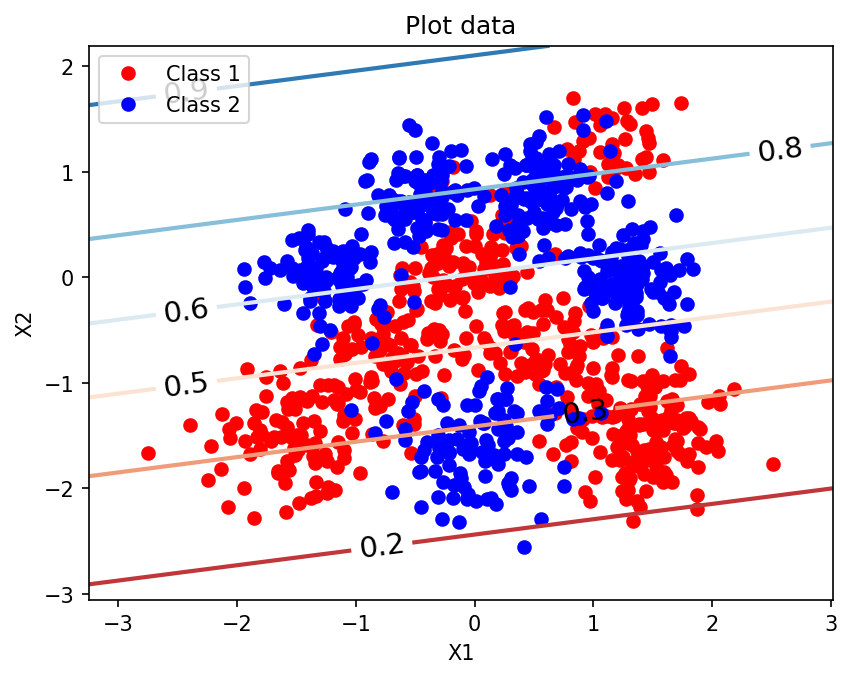
\includegraphics[width=0.25\paperwidth]{figures/contours_linear.png}
        \par\end{centering}
    \caption{Contours of the class predictive probabilities for the
        linear logistic classifier.\label{fig:contours_linear}}
\end{figure}


\section*{Exercise e) Log-Likelihoods and Confusion Matrix}

The final average training and test log-likelihoods are shown in
Table~\ref{tab:average_ll}. The test log-likelihood ($-0.6551$) is
slightly lower than the training log-likelihood ($-0.6161$), which is
expected since the model was fitted to the training data. The small gap
between them confirms the absence of significant overfitting.
However both values are close to $-\ln 2 \approx -0.693$, which is the
log-likelihood of a random coin-flip classifier, indicating that the
linear model offers only a modest improvement over random guessing on
this non-linearly separable dataset.

The $2 \times 2$ confusion matrix on the test set (using threshold
$\tau = 0.5$) is shown in Table~\ref{tab:confusion_test}.
The classifier correctly identifies 71.88\% of Class 1 ($y=1$) points
and 61.54\% of Class 0 ($y=0$) points. However, the error rates are
substantial: 38.46\% of true Class 0 points are misclassified as
Class 1, and 28.12\% of true Class 1 points are misclassified as
Class 0. This confirms that the linear decision boundary is inadequate
for this dataset.

\begin{table}[h]
    \centering{}%
    \begin{minipage}[t]{0.49\columnwidth}%
        \begin{center}
            \begin{tabular}{c|c}
                \textbf{Avg. Train ll} & \textbf{Avg. Test ll}\tabularnewline
                \hline
                $-0.6161$              & $-0.6551$\tabularnewline
                \hline
            \end{tabular}
            \par\end{center}
        \caption{Average training and test log-likelihoods for the linear
            classifier.\label{tab:average_ll}}
        %
    \end{minipage}%
    \begin{minipage}[t]{0.49\columnwidth}%
        \begin{center}
            \begin{tabular}{cc|c|c}
                    & \multicolumn{1}{c}{} & \multicolumn{1}{c}{$\hat{y}$} & \tabularnewline
                    &                      & 0                             & 1\tabularnewline
                \cline{2-4}
                $y$ & 0                    & 0.6154                        & 0.3846\tabularnewline
                \cline{2-4}
                    & 1                    & 0.2812                        & 0.7188\tabularnewline
                \cline{2-4}
            \end{tabular}
            \par\end{center}
        \caption{Confusion matrix on the test set (fractions conditioned on
            true label).\label{tab:confusion_test}}
        %
    \end{minipage}
\end{table}


\section*{Exercise f) Non-Linear Feature Expansion with RBFs}

To overcome the limitations of the linear classifier, we expand the
original two-dimensional inputs through a set of $N_{\text{train}}$
Gaussian radial basis functions (RBFs), each centred on one training
datapoint:
\[
    \tilde{\mathbf{x}}^{(n)}_{\text{RBF}}
    = \left(1,\; \phi_1(\mathbf{x}^{(n)}),\;
    \phi_2(\mathbf{x}^{(n)}),\; \ldots,\;
    \phi_{N_{\text{train}}}(\mathbf{x}^{(n)})\right)^T
    \in \mathbb{R}^{N_{\text{train}}+1}
\]
where each basis function $\phi_m$ is a Gaussian kernel centred on the
$m$-th training point $\mathbf{x}^{(m)}$:
\[
    \phi_m(\mathbf{x}^{(n)})
    = \exp\!\left(
    -\frac{1}{2l^2}\sum_{d=1}^{D}\left(x_d^{(n)} - x_d^{(m)}\right)^2
    \right)
    = \exp\!\left(
    -\frac{\|\mathbf{x}^{(n)} - \mathbf{x}^{(m)}\|^2}{2l^2}
    \right)
\]
The hyperparameter $l > 0$ is the \emph{width} of the
RBFs. Intuitively, $\phi_m(\mathbf{x}^{(n)})$ measures how close
$\mathbf{x}^{(n)}$ is to the $m$-th training centre: it equals $1$ when
$\mathbf{x}^{(n)} = \mathbf{x}^{(m)}$ and decays to $0$ as the
Euclidean distance $\|\mathbf{x}^{(n)} - \mathbf{x}^{(m)}\|$ grows
relative to $l$. The logistic classifier is now applied in this
$(N_{\text{train}}+1)$-dimensional feature space rather than the original
$(D+1)$-dimensional space.

\subsection*{Experimental Results}

We train the logistic classifier with RBF features for three widths
$l \in \{0.01, 0.1, 1\}$, using learning rates
$\eta \in \{0.0001, 0.001, 0.00005\}$ and $T = 500$ gradient ascent
steps for each, respectively.
The learning rates were chosen so that the log-likelihood
increases roughly monotonically without oscillation; Figure~\ref{fig:rbf_all} displays our results.

\begin{figure}[h]
    \centering
    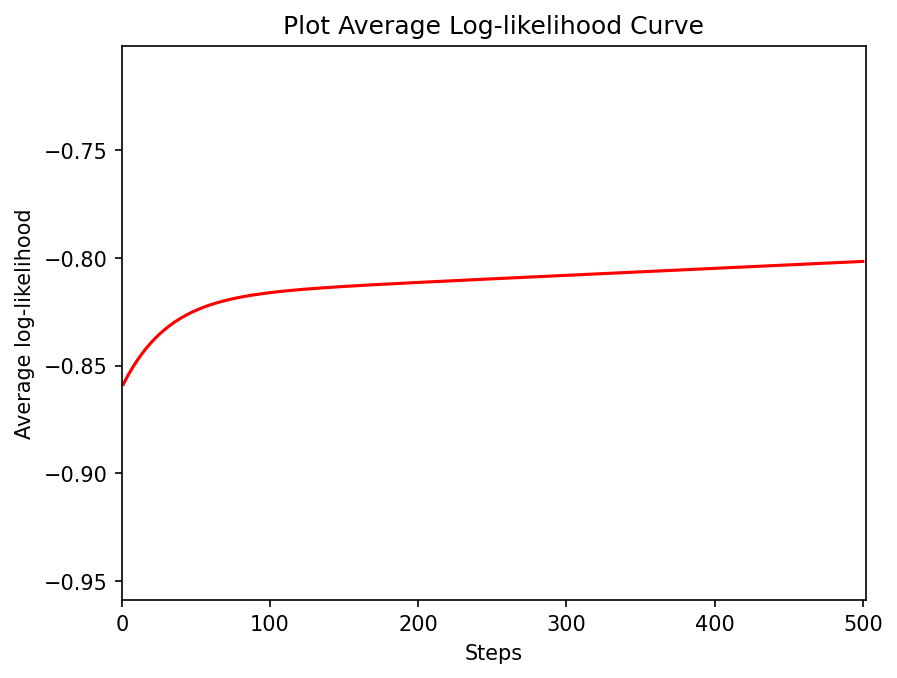
\includegraphics[width=0.23\textwidth]{figures/ll_train_rbf_0.01.png}\hspace{0cm}
    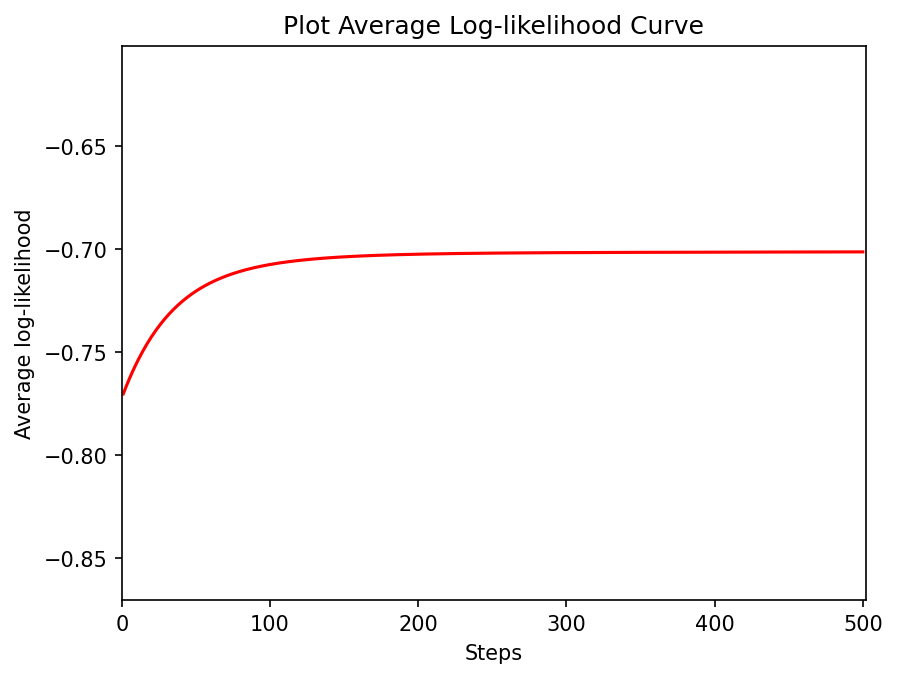
\includegraphics[width=0.23\textwidth]{figures/ll_test_rbf_0.01.png}\hspace{0cm}
    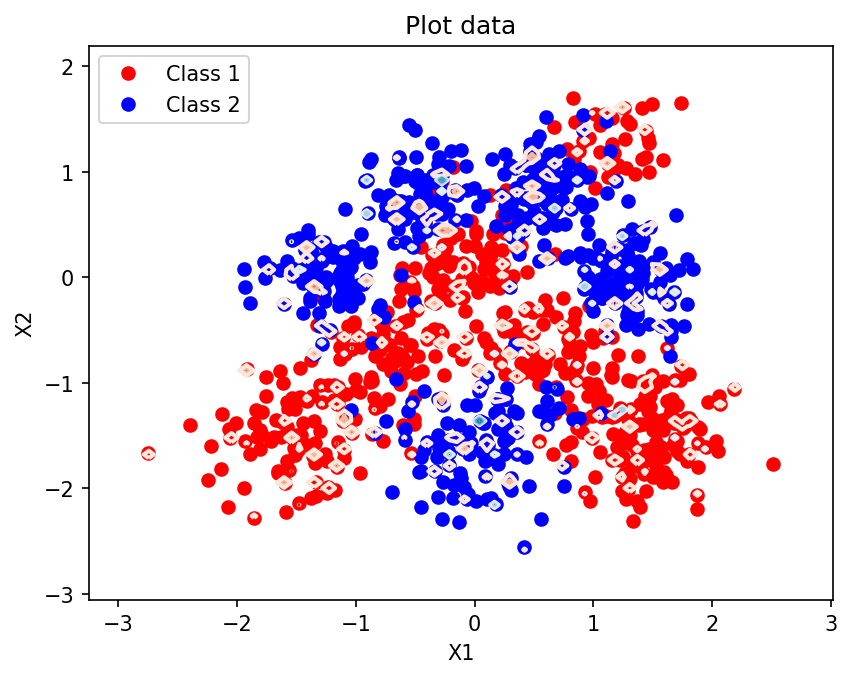
\includegraphics[width=0.23\textwidth]{figures/contours_rbf_0.01.png}\\[-0.1cm]
    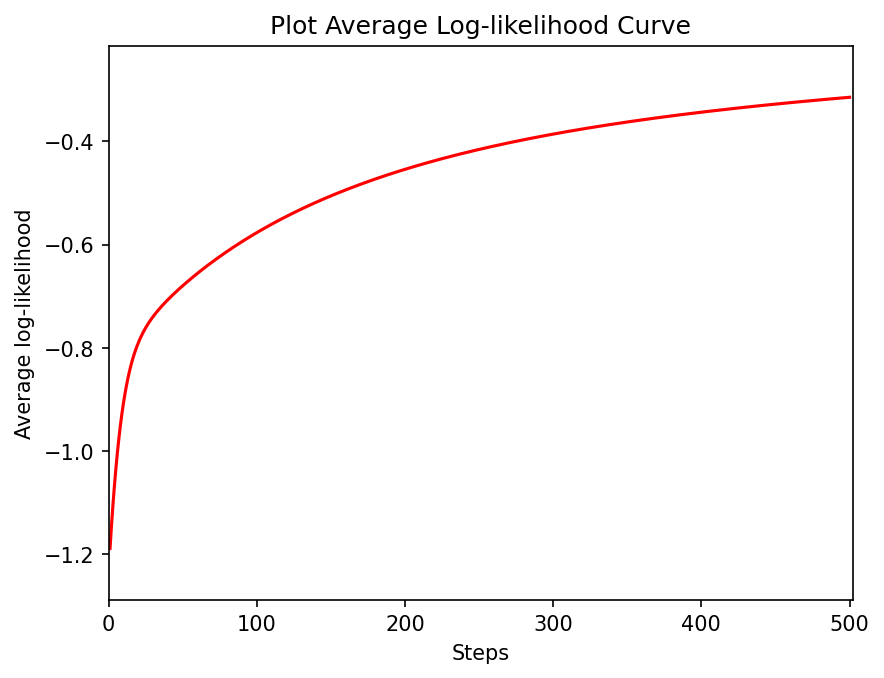
\includegraphics[width=0.23\textwidth]{figures/ll_train_rbf_0.1.png}\hspace{0cm}
    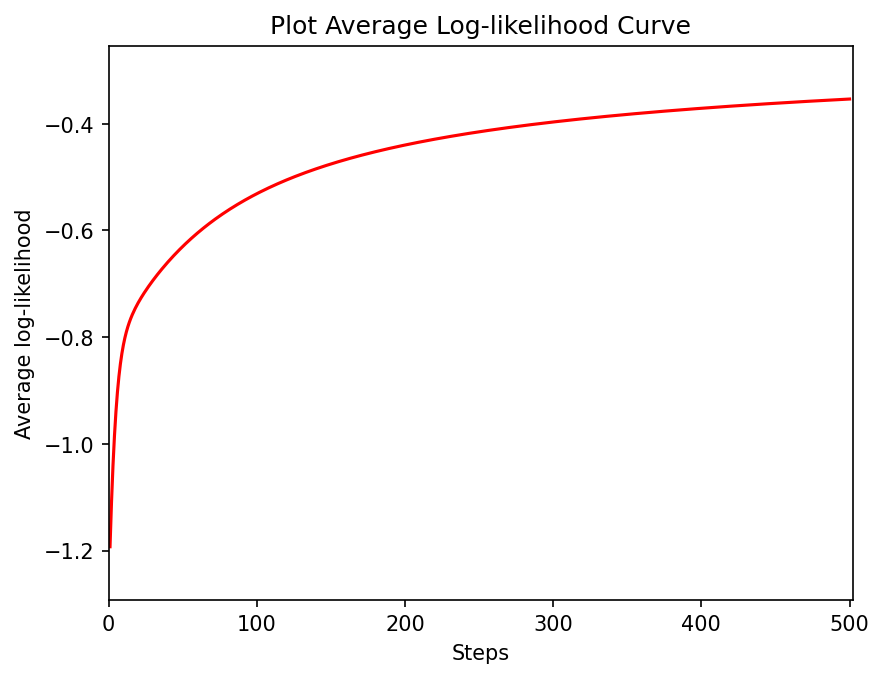
\includegraphics[width=0.23\textwidth]{figures/ll_test_rbf_0.1.png}\hspace{0cm}
    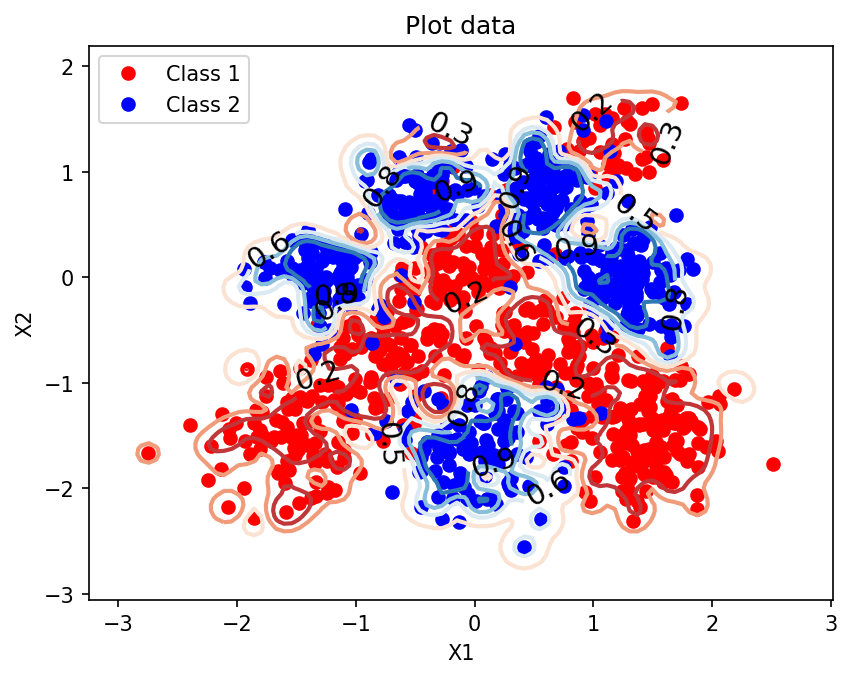
\includegraphics[width=0.23\textwidth]{figures/contours_rbf_0.1.png}\\[-0.1cm]
    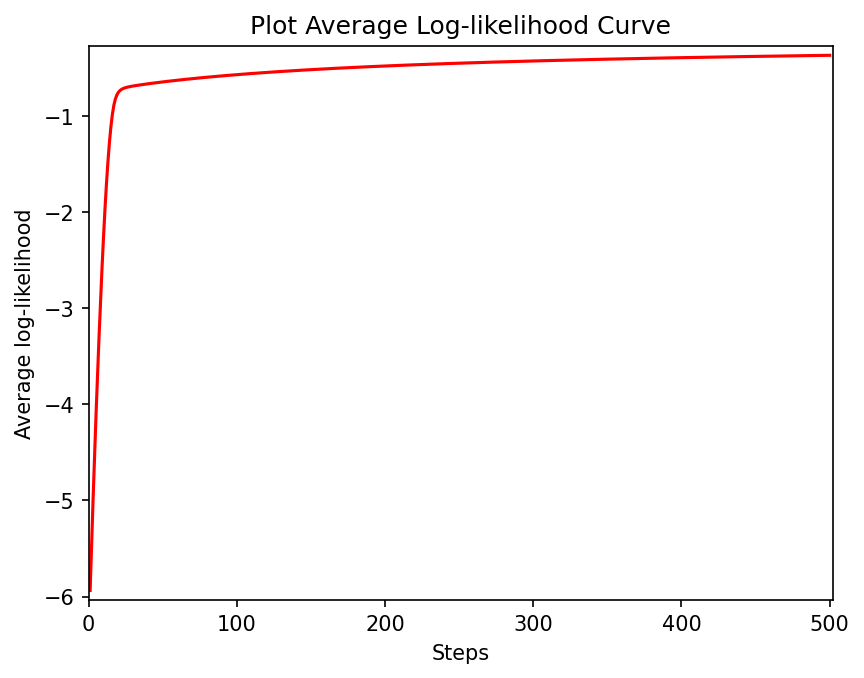
\includegraphics[width=0.23\textwidth]{figures/ll_train_rbf_1.0.png}\hspace{0cm}
    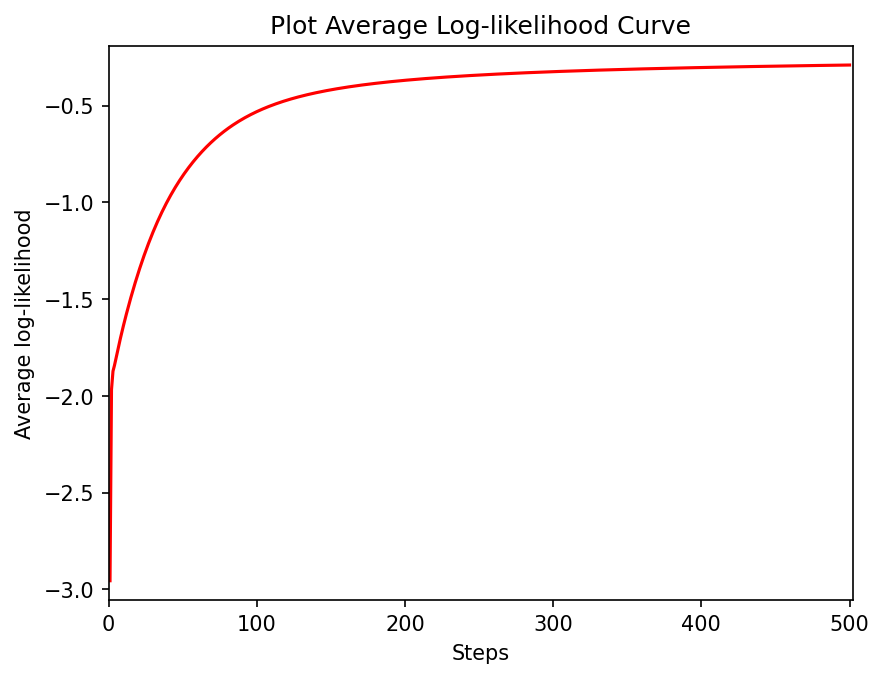
\includegraphics[width=0.23\textwidth]{figures/ll_test_rbf_1.0.png}\hspace{0cm}
    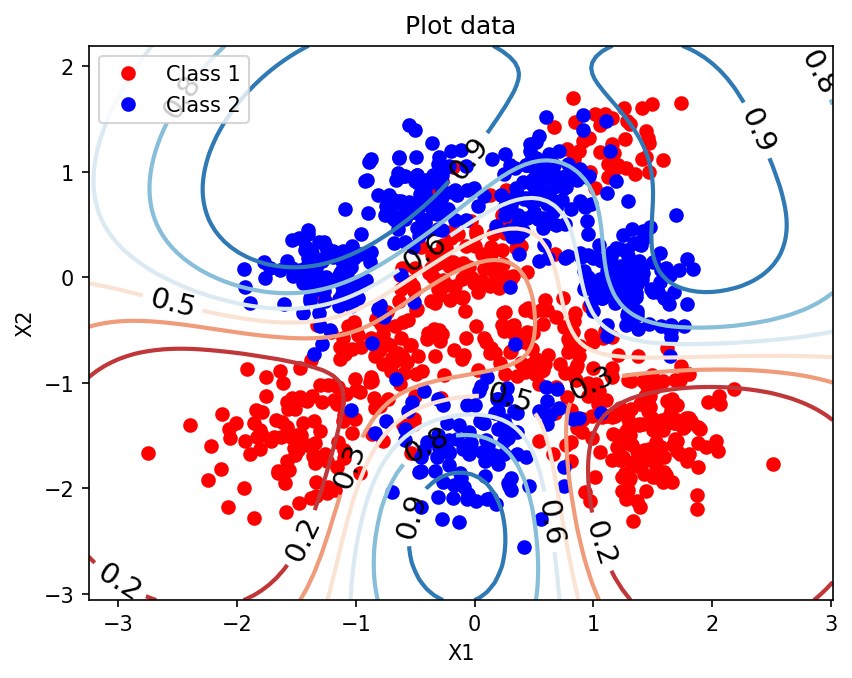
\includegraphics[width=0.23\textwidth]{figures/contours_rbf_1.0.png}
    \caption{Train log-likelihood (left), test log-likelihood (middle),
        and predictive contours (right).
        \textbf{Top:} $l = 0.01$, $\eta = 0.0001$.
        \textbf{Mid:} $l = 0.1$, $\eta = 0.001$.
        \textbf{Bot:} $l = 1.0$, $\eta = 0.00005$.
        All $T = 500$.
        \label{fig:rbf_all}}
\end{figure}

\subsection*{Discussion of results}

\subsubsection*{Role of the width $l$}

The width $l$ controls the \emph{smoothness} of the feature expansion
and thereby governs the bias--variance trade-off:

\begin{itemize}
    \item \textbf{Small $l$ (e.g.\ $l = 0.01$):}
          Each $\phi_m$ is extremely narrow -- essentially non-zero only
          at its own centre. The feature matrix approximates the identity,
          so the model cannot interpolate between training points (generalize beyond train set).
          The contours confirm this: predictions are highly localised spikes,
          and both test and train log-likelihoods are near $-\ln 2 \approx -0.693$, basically random guessing. Overfitting has clearly occurred.

    \item \textbf{Intermediate $l$ (e.g.\ $l = 0.1$):}
          Basis functions overlap enough for neighbouring points to share
          information, yet remain localised enough to capture non-linear
          structure. The contours show structured decision regions
          matching the true class distribution. Train/test log-likelihoods
          ($-0.2433$/$-0.3537$) are a substantial improvement over both
          the linear classifier and $l = 0.01$.

    \item \textbf{Large $l$ (e.g.\ $l = 1$):}
          Broad basis functions produce simpler (closer to linear) decision areas, where the contours are smooth and capture large-scale class structure well. Train/test log-likelihoods
          ($-0.3676$/$-0.4143$) show a small gap, indicating good
          generalisation. If $l$ is too large the model underfits.
\end{itemize}

Overall, increasing $l$ from $0.01$ to $1.0$ transitions the model
from overly localised (overfitting to training data) through
well-structured non-linear boundaries to smooth, close to linear decision boundaries.

\subsubsection*{Impact on the learning rate $\eta$}

For small $l$, the feature matrix approximates the identity with
small gradient magnitudes, so a moderate $\eta$ suffices. For
intermediate $l$, features overlap and gradient magnitudes grow, so a
larger $\eta$ speeds convergence. For large $l$, features are highly
correlated with large gradient magnitudes, demanding a smaller $\eta$ to avoid
divergence. Figure~\ref{fig:osc} demonstrates this: using
$\eta = 0.0005$ ($10\times$ larger) for $l = 1.0$ causes severe
oscillations as the gradient steps overshoot the optimum each iteration.

\begin{figure}[h]
    \centering
    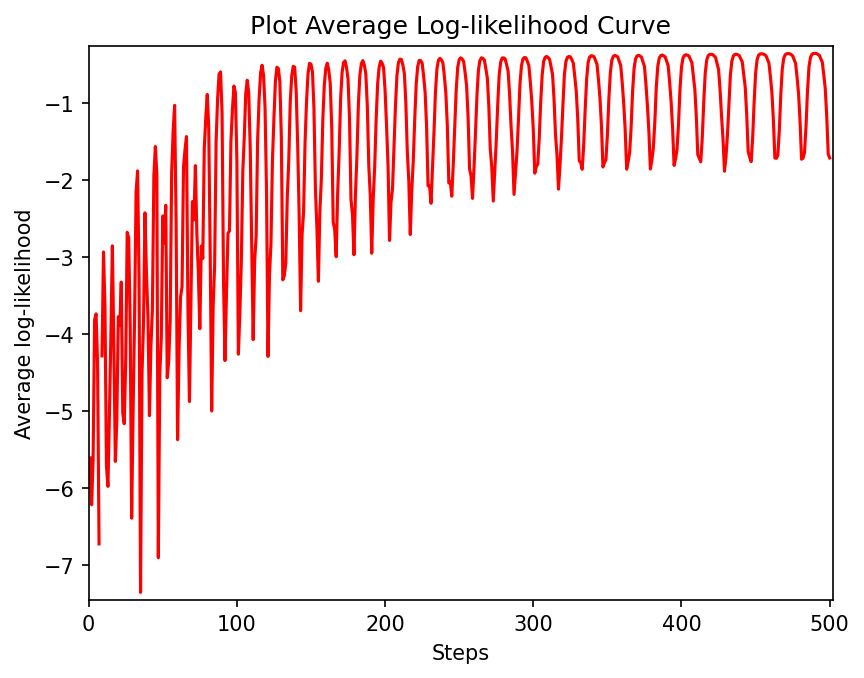
\includegraphics[width=0.27\textwidth]{figures/ll_train_rbf_1.0_osc.png}\hspace{0.2cm}
    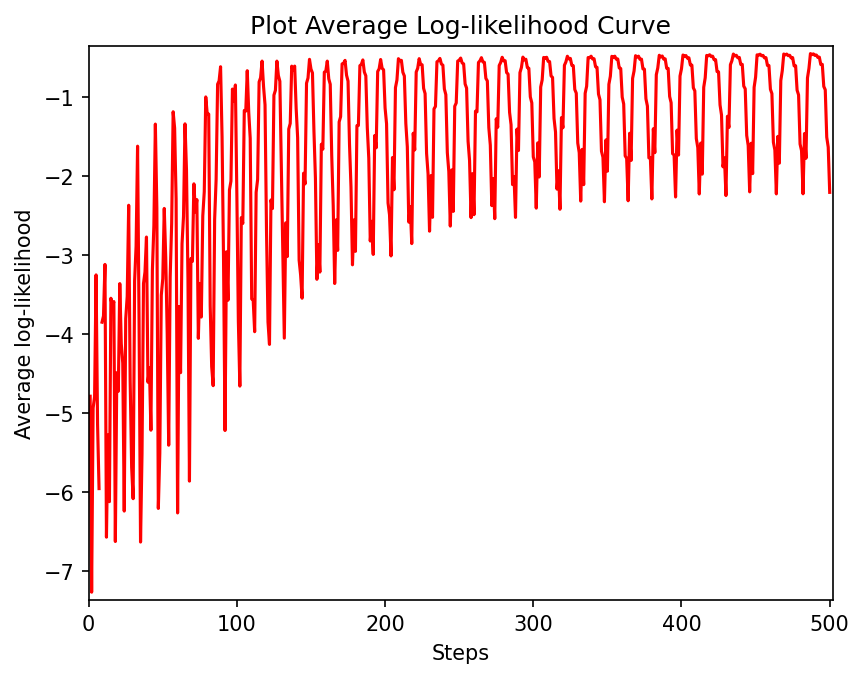
\includegraphics[width=0.27\textwidth]{figures/ll_test_rbf_1.0_osc.png}
    \caption{Train (left) and test (right) log-likelihood for $l = 1.0$ with $\eta = 0.0005$,
        demonstrating oscillations from an excessively large learning rate.\label{fig:osc}}
\end{figure}

\section*{Exercise g) Comparison of Results}

The final training and test log-likelihoods per datapoint for all four
models (linear and RBF with $l \in \{0.01, 0.1, 1\}$) are summarised
in Table~\ref{tab:all_ll}. The corresponding confusion matrices on the
test set (threshold $\tau = 0.5$) are shown in
Tables~\ref{tab:conf_linear}--\ref{tab:conf_l_1}.

\begin{table}[h]
    \centering
    \begin{tabular}{l|c|c}
        \textbf{Model} & \textbf{Avg. Train ll} & \textbf{Avg. Test ll} \\
        \hline
        Linear         & $-0.6161$              & $-0.6551$             \\
        RBF $l=0.01$   & $-0.7907$              & $-0.6927$             \\
        RBF $l=0.1$    & $-0.2433$              & $-0.3537$             \\
        RBF $l=1.0$    & $-0.3676$              & $-0.4143$             \\
    \end{tabular}
    \caption{Average log-likelihoods per datapoint for all models.\label{tab:all_ll}}
\end{table}

\begin{table}[h]
    \centering{}%
    \begin{minipage}[t]{0.24\textwidth}%
        \begin{center}
            \begin{tabular}{cc|c|c}
                    & \multicolumn{1}{c}{} & \multicolumn{2}{c}{$\hat{y}$} \tabularnewline
                    &                      & 0                                             & 1\tabularnewline
                \cline{2-4}
                $y$ & 0                    & 0.6154                                        & 0.3846\tabularnewline
                \cline{2-4}
                    & 1                    & 0.2812                                        & 0.7188\tabularnewline
                \cline{2-4}
            \end{tabular}
            \par\end{center}
        \caption{Conf. matrix, linear.\label{tab:conf_linear}}
    \end{minipage}\hfill%
    \begin{minipage}[t]{0.24\textwidth}%
        \begin{center}
            \begin{tabular}{cc|c|c}
                    & \multicolumn{1}{c}{} & \multicolumn{2}{c}{$\hat{y}$} \tabularnewline
                    &                      & 0                                             & 1\tabularnewline
                \cline{2-4}
                $y$ & 0                    & 0.9615                                        & 0.0385\tabularnewline
                \cline{2-4}
                    & 1                    & 0.9167                                        & 0.0833\tabularnewline
                \cline{2-4}
            \end{tabular}
            \par\end{center}
        \caption{Conf. matrix, $l=0.01$.\label{tab:conf_l_001}}
    \end{minipage}\hfill%
    \begin{minipage}[t]{0.24\textwidth}%
        \begin{center}
            \begin{tabular}{cc|c|c}
                    & \multicolumn{1}{c}{} & \multicolumn{2}{c}{$\hat{y}$} \tabularnewline
                    &                      & 0                                             & 1\tabularnewline
                \cline{2-4}
                $y$ & 0                    & 0.9327                                        & 0.0673\tabularnewline
                \cline{2-4}
                    & 1                    & 0.2083                                        & 0.7917\tabularnewline
                \cline{2-4}
            \end{tabular}
            \par\end{center}
        \caption{Conf. matrix, $l=0.1$.\label{tab:conf_l_01}}
    \end{minipage}\hfill%
    \begin{minipage}[t]{0.24\textwidth}%
        \begin{center}
            \begin{tabular}{cc|c|c}
                    & \multicolumn{1}{c}{} & \multicolumn{2}{c}{$\hat{y}$} \tabularnewline
                    &                      & 0                                             & 1\tabularnewline
                \cline{2-4}
                $y$ & 0                    & 0.7885                                        & 0.2115\tabularnewline
                \cline{2-4}
                    & 1                    & 0.1250                                        & 0.8750\tabularnewline
                \cline{2-4}
            \end{tabular}
            \par\end{center}
        \caption{Conf. matrix, $l=1$.\label{tab:conf_l_1}}
    \end{minipage}
\end{table}

The $l = 0.1$ model achieves the best test log-likelihood ($-0.3537$
vs.\ $-0.6551$ linear) with both high true negative ($0.93$) and true
positive ($0.79$) rates, reflecting its ability to capture non-linear
class structure. The $l = 1.0$ model has the best true positive rate
($0.875$) but a higher false positive rate ($0.21$), as its smooth
features lack resolution for finer boundaries. The $l = 0.01$ model
performs near random guessing (test ll $-0.6927$), with a confusion
matrix biased toward $\hat{y} = 0$ (true positive rate only $0.08$) because the
narrow basis functions mean test points almost always lie outside any decision boundaries - the model never predicts confidently for any class. Compared to the linear classifier, all RBF models reduce the false
positive rate ($0.38$ for linear). However, only $l = 0.1$ and $l = 1.0$
maintain a high true positive rate, confirming that an appropriately
chosen RBF width substantially improves classification.


\section*{Conclusions}

The linear logistic classifier achieves a test log-likelihood of
$-0.6551$, only marginally better than random guessing ($-\ln 2
    \approx -0.693$), confirming its inability to model the non-linear
class structure. Expanding the inputs with Gaussian RBFs yields substantial improvements:
$l = 0.1$ achieves the best test log-likelihood ($-0.3537$) with
balanced classification accuracy, while $l = 1.0$ achieves the
highest true positive rate at the cost of more false positives.
The RBF width $l$ controls the bias--variance trade-off: too small
gives overly localised features that fail to generalise, while too
large smooths away fine-grained class structure. Limitations include the lack of regularisation (which could mitigate overfitting for small $l$), and that the learning rates
were chosen by manual tuning rather than a systematic search.

\end{document}
